% $Header$

\documentclass{beamer}
%\documentclass[handout]{beamer}

\usepackage{amsmath,amssymb,latexsym,eucal,amsthm,graphicx,xcolor}
%%%%%%%%%%%%%%%%%%%%%%%%%%%%%%%%%%%%%%%%%%%%%
% Common Set Theory Constructs
%%%%%%%%%%%%%%%%%%%%%%%%%%%%%%%%%%%%%%%%%%%%%

\newcommand{\setof}[2]{\left\{ \, #1 \, \left| \, #2 \, \right.\right\}}
\newcommand{\lsetof}[2]{\left\{\left. \, #1 \, \right| \, #2 \,  \right\}}
\newcommand{\bigsetof}[2]{\bigl\{ \, #1 \, \bigm | \, #2 \,\bigr\}}
\newcommand{\Bigsetof}[2]{\Bigl\{ \, #1 \, \Bigm | \, #2 \,\Bigr\}}
\newcommand{\biggsetof}[2]{\biggl\{ \, #1 \, \biggm | \, #2 \,\biggr\}}
\newcommand{\Biggsetof}[2]{\Biggl\{ \, #1 \, \Biggm | \, #2 \,\Biggr\}}
\newcommand{\dotsetof}[2]{\left\{ \, #1 \, : \, #2 \, \right\}}
\newcommand{\bigdotsetof}[2]{\bigl\{ \, #1 \, : \, #2 \,\bigr\}}
\newcommand{\Bigdotsetof}[2]{\Bigl\{ \, #1 \, \Bigm : \, #2 \,\Bigr\}}
\newcommand{\biggdotsetof}[2]{\biggl\{ \, #1 \, \biggm : \, #2 \,\biggr\}}
\newcommand{\Biggdotsetof}[2]{\Biggl\{ \, #1 \, \Biggm : \, #2 \,\Biggr\}}
\newcommand{\sequence}[2]{\left\langle \, #1 \,\left| \, #2 \, \right. \right\rangle}
\newcommand{\lsequence}[2]{\left\langle\left. \, #1 \, \right| \,#2 \,  \right\rangle}
\newcommand{\bigsequence}[2]{\bigl\langle \,#1 \, \bigm | \, #2 \, \bigr\rangle}
\newcommand{\Bigsequence}[2]{\Bigl\langle \,#1 \, \Bigm | \, #2 \, \Bigr\rangle}
\newcommand{\biggsequence}[2]{\biggl\langle \,#1 \, \biggm | \, #2 \, \biggr\rangle}
\newcommand{\Biggsequence}[2]{\Biggl\langle \,#1 \, \Biggm | \, #2 \, \Biggr\rangle}
\newcommand{\singleton}[1]{\left\{#1\right\}}
\newcommand{\angles}[1]{\left\langle #1 \right\rangle}
\newcommand{\bigangles}[1]{\bigl\langle #1 \bigr\rangle}
\newcommand{\Bigangles}[1]{\Bigl\langle #1 \Bigr\rangle}
\newcommand{\biggangles}[1]{\biggl\langle #1 \biggr\rangle}
\newcommand{\Biggangles}[1]{\Biggl\langle #1 \Biggr\rangle}


\newcommand{\force}[1]{\Vert\!\underset{\!\!\!\!\!#1}{\!\!\!\relbar\!\!\!%
\relbar\!\!\relbar\!\!\relbar\!\!\!\relbar\!\!\relbar\!\!\relbar\!\!\!%
\relbar\!\!\relbar\!\!\relbar}}
\newcommand{\longforce}[1]{\Vert\!\underset{\!\!\!\!\!#1}{\!\!\!\relbar\!\!\!%
\relbar\!\!\relbar\!\!\relbar\!\!\!\relbar\!\!\relbar\!\!\relbar\!\!\!%
\relbar\!\!\relbar\!\!\relbar\!\!\relbar\!\!\relbar\!\!\relbar\!\!\relbar\!\!\relbar}}
\newcommand{\nforce}[1]{\Vert\!\underset{\!\!\!\!\!#1}{\!\!\!\relbar\!\!\!%
\relbar\!\!\relbar\!\!\relbar\!\!\!\relbar\!\!\relbar\!\!\relbar\!\!\!%
\relbar\!\!\not\relbar\!\!\relbar}}
\newcommand{\forcein}[2]{\overset{#2}{\Vert\underset{\!\!\!\!\!#1}%
{\!\!\!\relbar\!\!\!\relbar\!\!\relbar\!\!\relbar\!\!\!\relbar\!\!\relbar\!%
\!\relbar\!\!\!\relbar\!\!\relbar\!\!\relbar\!\!\relbar\!\!\!\relbar\!\!%
\relbar\!\!\relbar}}}

\newcommand{\pre}[2]{{}^{#2}{#1}}

\newcommand{\restr}{\!\!\upharpoonright\!}

%%%%%%%%%%%%%%%%%%%%%%%%%%%%%%%%%%%%%%%%%%%%%
% Set-Theoretic Connectives
%%%%%%%%%%%%%%%%%%%%%%%%%%%%%%%%%%%%%%%%%%%%%

\newcommand{\intersect}{\cap}
\newcommand{\union}{\cup}
\newcommand{\Intersection}[1]{\bigcap\limits_{#1}}
\newcommand{\Union}[1]{\bigcup\limits_{#1}}
\newcommand{\adjoin}{{}^\frown}
\newcommand{\forces}{\Vdash}

%%%%%%%%%%%%%%%%%%%%%%%%%%%%%%%%%%%%%%%%%%%%%
% Miscellaneous
%%%%%%%%%%%%%%%%%%%%%%%%%%%%%%%%%%%%%%%%%%%%%
\newcommand{\defeq}{=_{\text{def}}}
\newcommand{\Turingleq}{\leq_{\text{T}}}
\newcommand{\Turingless}{<_{\text{T}}}
\newcommand{\lexleq}{\leq_{\text{lex}}}
\newcommand{\lexless}{<_{\text{lex}}}
\newcommand{\Turingequiv}{\equiv_{\text{T}}}
\newcommand{\isomorphic}{\cong}

%%%%%%%%%%%%%%%%%%%%%%%%%%%%%%%%%%%%%%%%%%%%%
% Constants
%%%%%%%%%%%%%%%%%%%%%%%%%%%%%%%%%%%%%%%%%%%%%
\newcommand{\R}{\mathbb{R}}
\renewcommand{\P}{\mathbb{P}}
\newcommand{\Q}{\mathbb{Q}}
\newcommand{\Z}{\mathbb{Z}}
\newcommand{\Zpos}{\Z^{+}}
\newcommand{\Znonneg}{\Z^{\geq 0}}
\newcommand{\C}{\mathbb{C}}
\newcommand{\N}{\mathbb{N}}
\newcommand{\B}{\mathbb{B}}
\newcommand{\Bairespace}{\pre{\omega}{\omega}}
\newcommand{\LofR}{L(\R)}
\newcommand{\JofR}[1]{J_{#1}(\R)}
\newcommand{\SofR}[1]{S_{#1}(\R)}
\newcommand{\JalphaR}{\JofR{\alpha}}
\newcommand{\JbetaR}{\JofR{\beta}}
\newcommand{\JlambdaR}{\JofR{\lambda}}
\newcommand{\SalphaR}{\SofR{\alpha}}
\newcommand{\SbetaR}{\SofR{\beta}}
\newcommand{\Pkl}{\mathcal{P}_{\kappa}(\lambda)}
\DeclareMathOperator{\con}{con}
\DeclareMathOperator{\ORD}{OR}
\DeclareMathOperator{\Ord}{OR}
\DeclareMathOperator{\WO}{WO}
\DeclareMathOperator{\OD}{OD}
\DeclareMathOperator{\HOD}{HOD}
\DeclareMathOperator{\HC}{HC}
\DeclareMathOperator{\WF}{WF}
\DeclareMathOperator{\wfp}{wfp}
\DeclareMathOperator{\HF}{HF}
\newcommand{\One}{I}
\newcommand{\ONE}{I}
\newcommand{\Two}{II}
\newcommand{\TWO}{II}
\newcommand{\Mladder}{M^{\text{ld}}}

%%%%%%%%%%%%%%%%%%%%%%%%%%%%%%%%%%%%%%%%%%%%%
% Commutative Algebra Constants
%%%%%%%%%%%%%%%%%%%%%%%%%%%%%%%%%%%%%%%%%%%%%
\DeclareMathOperator{\dottimes}{\dot{\times}}
\DeclareMathOperator{\dotminus}{\dot{-}}
\DeclareMathOperator{\Spec}{Spec}

%%%%%%%%%%%%%%%%%%%%%%%%%%%%%%%%%%%%%%%%%%%%%
% Theories
%%%%%%%%%%%%%%%%%%%%%%%%%%%%%%%%%%%%%%%%%%%%%
\DeclareMathOperator{\ZFC}{ZFC}
\DeclareMathOperator{\ZF}{ZF}
\DeclareMathOperator{\AD}{AD}
\DeclareMathOperator{\ADR}{AD_{\R}}
\DeclareMathOperator{\KP}{KP}
\DeclareMathOperator{\PD}{PD}
\DeclareMathOperator{\CH}{CH}
\DeclareMathOperator{\GCH}{GCH}
\DeclareMathOperator{\HPC}{HPC} % HOD pair capturing
%%%%%%%%%%%%%%%%%%%%%%%%%%%%%%%%%%%%%%%%%%%%%
% Iteration Trees
%%%%%%%%%%%%%%%%%%%%%%%%%%%%%%%%%%%%%%%%%%%%%

\newcommand{\pred}{\text{-pred}}

%%%%%%%%%%%%%%%%%%%%%%%%%%%%%%%%%%%%%%%%%%%%%%%%
% Operator Names
%%%%%%%%%%%%%%%%%%%%%%%%%%%%%%%%%%%%%%%%%%%%%%%%
\DeclareMathOperator{\Det}{Det}
\DeclareMathOperator{\dom}{dom}
\DeclareMathOperator{\ran}{ran}
\DeclareMathOperator{\range}{ran}
\DeclareMathOperator{\image}{image}
\DeclareMathOperator{\crit}{crit}
\DeclareMathOperator{\card}{card}
\DeclareMathOperator{\cf}{cf}
\DeclareMathOperator{\cof}{cof}
\DeclareMathOperator{\rank}{rank}
\DeclareMathOperator{\ot}{o.t.}
\DeclareMathOperator{\ords}{o}
\DeclareMathOperator{\ro}{r.o.}
\DeclareMathOperator{\rud}{rud}
\DeclareMathOperator{\Powerset}{\mathcal{P}}
\DeclareMathOperator{\length}{lh}
\DeclareMathOperator{\lh}{lh}
\DeclareMathOperator{\limit}{lim}
\DeclareMathOperator{\fld}{fld}
\DeclareMathOperator{\projection}{p}
\DeclareMathOperator{\Ult}{Ult}
\DeclareMathOperator{\ULT}{Ult}
\DeclareMathOperator{\Coll}{Coll}
\DeclareMathOperator{\Col}{Col}
\DeclareMathOperator{\Hull}{Hull}
\DeclareMathOperator*{\dirlim}{dir lim}
\DeclareMathOperator{\Scale}{Scale}
\DeclareMathOperator{\supp}{supp}
\DeclareMathOperator{\trancl}{tran.cl.}
\DeclareMathOperator{\trace}{Tr}
\DeclareMathOperator{\diag}{diag}
\DeclareMathOperator{\spn}{span}
\DeclareMathOperator{\sgn}{sgn}
%%%%%%%%%%%%%%%%%%%%%%%%%%%%%%%%%%%%%%%%%%%%%
% Logical Connectives
%%%%%%%%%%%%%%%%%%%%%%%%%%%%%%%%%%%%%%%%%%%%%
\newcommand{\IImplies}{\Longrightarrow}
\newcommand{\SkipImplies}{\quad\Longrightarrow\quad}
\newcommand{\Ifff}{\Longleftrightarrow}
\newcommand{\iimplies}{\longrightarrow}
\newcommand{\ifff}{\longleftrightarrow}
\newcommand{\Implies}{\Rightarrow}
\newcommand{\Iff}{\Leftrightarrow}
\renewcommand{\implies}{\rightarrow}
\renewcommand{\iff}{\leftrightarrow}
\newcommand{\AND}{\wedge}
\newcommand{\OR}{\vee}
\newcommand{\st}{\text{ s.t. }}
\newcommand{\Or}{\text{ or }}

%%%%%%%%%%%%%%%%%%%%%%%%%%%%%%%%%%%%%%%%%%%%%
% Function Arrows
%%%%%%%%%%%%%%%%%%%%%%%%%%%%%%%%%%%%%%%%%%%%%

\newcommand{\injection}{\xrightarrow{\text{1-1}}}
\newcommand{\surjection}{\xrightarrow{\text{onto}}}
\newcommand{\bijection}{\xrightarrow[\text{onto}]{\text{1-1}}}
\newcommand{\cofmap}{\xrightarrow{\text{cof}}}
\newcommand{\map}{\rightarrow}

%%%%%%%%%%%%%%%%%%%%%%%%%%%%%%%%%%%%%%%%%%%%%
% Mouse Comparison Operators
%%%%%%%%%%%%%%%%%%%%%%%%%%%%%%%%%%%%%%%%%%%%%
\newcommand{\initseg}{\trianglelefteq}
\newcommand{\properseg}{\lhd}
\newcommand{\notinitseg}{\ntrianglelefteq}
\newcommand{\notproperseg}{\ntriangleleft}

%%%%%%%%%%%%%%%%%%%%%%%%%%%%%%%%%%%%%%%%%%%%%
%           calligraphic letters
%%%%%%%%%%%%%%%%%%%%%%%%%%%%%%%%%%%%%%%%%%%%%
\newcommand{\cA}{\mathcal{A}}
\newcommand{\cB}{\mathcal{B}}
\newcommand{\cC}{\mathcal{C}}
\newcommand{\cD}{\mathcal{D}}
\newcommand{\cE}{\mathcal{E}}
\newcommand{\cF}{\mathcal{F}}
\newcommand{\cG}{\mathcal{G}}
\newcommand{\cH}{\mathcal{H}}
\newcommand{\cI}{\mathcal{I}}
\newcommand{\cJ}{\mathcal{J}}
\newcommand{\cK}{\mathcal{K}}
\newcommand{\cL}{\mathcal{L}}
\newcommand{\cM}{\mathcal{M}}
\newcommand{\cN}{\mathcal{N}}
\newcommand{\cO}{\mathcal{O}}
\newcommand{\cP}{\mathcal{P}}
\newcommand{\cQ}{\mathcal{Q}}
\newcommand{\cR}{\mathcal{R}}
\newcommand{\cS}{\mathcal{S}}
\newcommand{\cT}{\mathcal{T}}
\newcommand{\cU}{\mathcal{U}}
\newcommand{\cV}{\mathcal{V}}
\newcommand{\cW}{\mathcal{W}}
\newcommand{\cX}{\mathcal{X}}
\newcommand{\cY}{\mathcal{Y}}
\newcommand{\cZ}{\mathcal{Z}}


%%%%%%%%%%%%%%%%%%%%%%%%%%%%%%%%%%%%%%%%%%%%%
%          Primed Letters
%%%%%%%%%%%%%%%%%%%%%%%%%%%%%%%%%%%%%%%%%%%%%
\newcommand{\aprime}{a^{\prime}}
\newcommand{\bprime}{b^{\prime}}
\newcommand{\cprime}{c^{\prime}}
\newcommand{\dprime}{d^{\prime}}
\newcommand{\eprime}{e^{\prime}}
\newcommand{\fprime}{f^{\prime}}
\newcommand{\gprime}{g^{\prime}}
\newcommand{\hprime}{h^{\prime}}
\newcommand{\iprime}{i^{\prime}}
\newcommand{\jprime}{j^{\prime}}
\newcommand{\kprime}{k^{\prime}}
\newcommand{\lprime}{l^{\prime}}
\newcommand{\mprime}{m^{\prime}}
\newcommand{\nprime}{n^{\prime}}
\newcommand{\oprime}{o^{\prime}}
\newcommand{\pprime}{p^{\prime}}
\newcommand{\qprime}{q^{\prime}}
\newcommand{\rprime}{r^{\prime}}
\newcommand{\sprime}{s^{\prime}}
\newcommand{\tprime}{t^{\prime}}
\newcommand{\uprime}{u^{\prime}}
\newcommand{\vprime}{v^{\prime}}
\newcommand{\wprime}{w^{\prime}}
\newcommand{\xprime}{x^{\prime}}
\newcommand{\yprime}{y^{\prime}}
\newcommand{\zprime}{z^{\prime}}
\newcommand{\Aprime}{A^{\prime}}
\newcommand{\Bprime}{B^{\prime}}
\newcommand{\Cprime}{C^{\prime}}
\newcommand{\Dprime}{D^{\prime}}
\newcommand{\Eprime}{E^{\prime}}
\newcommand{\Fprime}{F^{\prime}}
\newcommand{\Gprime}{G^{\prime}}
\newcommand{\Hprime}{H^{\prime}}
\newcommand{\Iprime}{I^{\prime}}
\newcommand{\Jprime}{J^{\prime}}
\newcommand{\Kprime}{K^{\prime}}
\newcommand{\Lprime}{L^{\prime}}
\newcommand{\Mprime}{M^{\prime}}
\newcommand{\Nprime}{N^{\prime}}
\newcommand{\Oprime}{O^{\prime}}
\newcommand{\Pprime}{P^{\prime}}
\newcommand{\Qprime}{Q^{\prime}}
\newcommand{\Rprime}{R^{\prime}}
\newcommand{\Sprime}{S^{\prime}}
\newcommand{\Tprime}{T^{\prime}}
\newcommand{\Uprime}{U^{\prime}}
\newcommand{\Vprime}{V^{\prime}}
\newcommand{\Wprime}{W^{\prime}}
\newcommand{\Xprime}{X^{\prime}}
\newcommand{\Yprime}{Y^{\prime}}
\newcommand{\Zprime}{Z^{\prime}}
\newcommand{\alphaprime}{\alpha^{\prime}}
\newcommand{\betaprime}{\beta^{\prime}}
\newcommand{\gammaprime}{\gamma^{\prime}}
\newcommand{\Gammaprime}{\Gamma^{\prime}}
\newcommand{\deltaprime}{\delta^{\prime}}
\newcommand{\epsilonprime}{\epsilon^{\prime}}
\newcommand{\kappaprime}{\kappa^{\prime}}
\newcommand{\lambdaprime}{\lambda^{\prime}}
\newcommand{\rhoprime}{\rho^{\prime}}
\newcommand{\Sigmaprime}{\Sigma^{\prime}}
\newcommand{\tauprime}{\tau^{\prime}}
\newcommand{\xiprime}{\xi^{\prime}}
\newcommand{\thetaprime}{\theta^{\prime}}
\newcommand{\Omegaprime}{\Omega^{\prime}}
\newcommand{\cMprime}{\cM^{\prime}}
\newcommand{\cNprime}{\cN^{\prime}}
\newcommand{\cPprime}{\cP^{\prime}}
\newcommand{\cQprime}{\cQ^{\prime}}
\newcommand{\cRprime}{\cR^{\prime}}
\newcommand{\cSprime}{\cS^{\prime}}
\newcommand{\cTprime}{\cT^{\prime}}

%%%%%%%%%%%%%%%%%%%%%%%%%%%%%%%%%%%%%%%%%%%%%
%          bar Letters
%%%%%%%%%%%%%%%%%%%%%%%%%%%%%%%%%%%%%%%%%%%%%
\newcommand{\abar}{\bar{a}}
\newcommand{\bbar}{\bar{b}}
\newcommand{\cbar}{\bar{c}}
\newcommand{\ibar}{\bar{i}}
\newcommand{\jbar}{\bar{j}}
\newcommand{\nbar}{\bar{n}}
\newcommand{\xbar}{\bar{x}}
\newcommand{\ybar}{\bar{y}}
\newcommand{\zbar}{\bar{z}}
\newcommand{\pibar}{\bar{\pi}}
\newcommand{\phibar}{\bar{\varphi}}
\newcommand{\psibar}{\bar{\psi}}
\newcommand{\thetabar}{\bar{\theta}}
\newcommand{\nubar}{\bar{\nu}}

%%%%%%%%%%%%%%%%%%%%%%%%%%%%%%%%%%%%%%%%%%%%%
%          star Letters
%%%%%%%%%%%%%%%%%%%%%%%%%%%%%%%%%%%%%%%%%%%%%
\newcommand{\phistar}{\phi^{*}}
\newcommand{\Mstar}{M^{*}}

%%%%%%%%%%%%%%%%%%%%%%%%%%%%%%%%%%%%%%%%%%%%%
%          dotletters Letters
%%%%%%%%%%%%%%%%%%%%%%%%%%%%%%%%%%%%%%%%%%%%%
\newcommand{\Gdot}{\dot{G}}

%%%%%%%%%%%%%%%%%%%%%%%%%%%%%%%%%%%%%%%%%%%%%
%         check Letters
%%%%%%%%%%%%%%%%%%%%%%%%%%%%%%%%%%%%%%%%%%%%%
\newcommand{\deltacheck}{\check{\delta}}
\newcommand{\gammacheck}{\check{\gamma}}


%%%%%%%%%%%%%%%%%%%%%%%%%%%%%%%%%%%%%%%%%%%%%
%          Formulas
%%%%%%%%%%%%%%%%%%%%%%%%%%%%%%%%%%%%%%%%%%%%%

\newcommand{\formulaphi}{\text{\large $\varphi$}}
\newcommand{\Formulaphi}{\text{\Large $\varphi$}}


%%%%%%%%%%%%%%%%%%%%%%%%%%%%%%%%%%%%%%%%%%%%%
%          Fraktur Letters
%%%%%%%%%%%%%%%%%%%%%%%%%%%%%%%%%%%%%%%%%%%%%

\newcommand{\fa}{\mathfrak{a}}
\newcommand{\fb}{\mathfrak{b}}
\newcommand{\fc}{\mathfrak{c}}
\newcommand{\fk}{\mathfrak{k}}
\newcommand{\fp}{\mathfrak{p}}
\newcommand{\fq}{\mathfrak{q}}
\newcommand{\fr}{\mathfrak{r}}
\newcommand{\fA}{\mathfrak{A}}
\newcommand{\fB}{\mathfrak{B}}
\newcommand{\fC}{\mathfrak{C}}
\newcommand{\fD}{\mathfrak{D}}

%%%%%%%%%%%%%%%%%%%%%%%%%%%%%%%%%%%%%%%%%%%%%
%          Bold Letters
%%%%%%%%%%%%%%%%%%%%%%%%%%%%%%%%%%%%%%%%%%%%%
\newcommand{\ba}{\mathbf{a}}
\newcommand{\bb}{\mathbf{b}}
\newcommand{\bc}{\mathbf{c}}
\newcommand{\bd}{\mathbf{d}}
\newcommand{\be}{\mathbf{e}}
\newcommand{\bu}{\mathbf{u}}
\newcommand{\bv}{\mathbf{v}}
\newcommand{\bw}{\mathbf{w}}
\newcommand{\bx}{\mathbf{x}}
\newcommand{\by}{\mathbf{y}}
\newcommand{\bz}{\mathbf{z}}
\newcommand{\bSigma}{\boldsymbol{\Sigma}}
\newcommand{\bPi}{\boldsymbol{\Pi}}
\newcommand{\bDelta}{\boldsymbol{\Delta}}
\newcommand{\bdelta}{\boldsymbol{\delta}}
\newcommand{\bgamma}{\boldsymbol{\gamma}}
\newcommand{\bGamma}{\boldsymbol{\Gamma}}

%%%%%%%%%%%%%%%%%%%%%%%%%%%%%%%%%%%%%%%%%%%%%
%         Bold numbers
%%%%%%%%%%%%%%%%%%%%%%%%%%%%%%%%%%%%%%%%%%%%%
\newcommand{\bzero}{\mathbf{0}}

%%%%%%%%%%%%%%%%%%%%%%%%%%%%%%%%%%%%%%%%%%%%%
% Projective-Like Pointclasses
%%%%%%%%%%%%%%%%%%%%%%%%%%%%%%%%%%%%%%%%%%%%%
\newcommand{\Sa}[2][\alpha]{\Sigma_{(#1,#2)}}
\newcommand{\Pa}[2][\alpha]{\Pi_{(#1,#2)}}
\newcommand{\Da}[2][\alpha]{\Delta_{(#1,#2)}}
\newcommand{\Aa}[2][\alpha]{A_{(#1,#2)}}
\newcommand{\Ca}[2][\alpha]{C_{(#1,#2)}}
\newcommand{\Qa}[2][\alpha]{Q_{(#1,#2)}}
\newcommand{\da}[2][\alpha]{\delta_{(#1,#2)}}
\newcommand{\leqa}[2][\alpha]{\leq_{(#1,#2)}}
\newcommand{\lessa}[2][\alpha]{<_{(#1,#2)}}
\newcommand{\equiva}[2][\alpha]{\equiv_{(#1,#2)}}


\newcommand{\Sl}[1]{\Sa[\lambda]{#1}}
\newcommand{\Pl}[1]{\Pa[\lambda]{#1}}
\newcommand{\Dl}[1]{\Da[\lambda]{#1}}
\newcommand{\Al}[1]{\Aa[\lambda]{#1}}
\newcommand{\Cl}[1]{\Ca[\lambda]{#1}}
\newcommand{\Ql}[1]{\Qa[\lambda]{#1}}

\newcommand{\San}{\Sa{n}}
\newcommand{\Pan}{\Pa{n}}
\newcommand{\Dan}{\Da{n}}
\newcommand{\Can}{\Ca{n}}
\newcommand{\Qan}{\Qa{n}}
\newcommand{\Aan}{\Aa{n}}
\newcommand{\dan}{\da{n}}
\newcommand{\leqan}{\leqa{n}}
\newcommand{\lessan}{\lessa{n}}
\newcommand{\equivan}{\equiva{n}}

\newcommand{\SigmaOneOmega}{\Sigma^1_{\omega}}
\newcommand{\SigmaOneOmegaPlusOne}{\Sigma^1_{\omega+1}}
\newcommand{\PiOneOmega}{\Pi^1_{\omega}}
\newcommand{\PiOneOmegaPlusOne}{\Pi^1_{\omega+1}}
\newcommand{\DeltaOneOmegaPlusOne}{\Delta^1_{\omega+1}}

%%%%%%%%%%%%%%%%%%%%%%%%%%%%%%%%%%%%%%%%%%%%%
% Linear Algebra
%%%%%%%%%%%%%%%%%%%%%%%%%%%%%%%%%%%%%%%%%%%%%
\newcommand{\transpose}[1]{{#1}^{\text{T}}}
\newcommand{\norm}[1]{\lVert{#1}\rVert}
\newcommand\aug{\fboxsep=-\fboxrule\!\!\!\fbox{\strut}\!\!\!}

%%%%%%%%%%%%%%%%%%%%%%%%%%%%%%%%%%%%%%%%%%%%%
% Number Theory
%%%%%%%%%%%%%%%%%%%%%%%%%%%%%%%%%%%%%%%%%%%%%
\newcommand{\av}[1]{\lvert#1\rvert}
\DeclareMathOperator{\divides}{\mid}
\DeclareMathOperator{\ndivides}{\nmid}
\DeclareMathOperator{\lcm}{lcm}
\DeclareMathOperator{\sign}{sign}
\newcommand{\floor}[1]{\left\lfloor{#1}\right\rfloor}
\DeclareMathOperator{\ConCl}{CC}
\DeclareMathOperator{\ord}{ord}



\graphicspath{{images/}}

\newtheorem*{claim}{claim}
\newtheorem*{observation}{Observation}
\newtheorem*{warning}{Warning}
\newtheorem*{question}{Question}
\newtheorem{remark}[theorem]{Remark}

\newenvironment*{subproof}[1][Proof]
{\begin{proof}[#1]}{\renewcommand{\qedsymbol}{$\diamondsuit$} \end{proof}}

\mode<presentation>
{
  \usetheme{Singapore}
  % or ...

  \setbeamercovered{invisible}
  % or whatever (possibly just delete it)
}


\usepackage[english]{babel}
% or whatever

\usepackage[latin1]{inputenc}
% or whatever

\usepackage{times}
\usepackage[T1]{fontenc}
% Or whatever. Note that the encoding and the font should match. If T1
% does not look nice, try deleting the line with the fontenc.

\title{Lesson 19 \\ Eigenvalues and Eigenvectors}
\subtitle{Math 325, Linear Algebra \\ Spring 2019 \\ SFSU}
\author{Mitch Rudominer}
\date{}



% If you wish to uncover everything in a step-wise fashion, uncomment
% the following command:

\beamerdefaultoverlayspecification{<+->}

\begin{document}

\begin{frame}
  \titlepage
\end{frame}

%%%%%%%%%%%%%%%%%%%%%%%%%%%%%%%%%%%%%%%%%%%%%%%%%%%%%%%%%%%%%%%%%%%%%%%%%

\begin{frame}{Eigen Pairs}

\begin{itemize}
\item \textbf{Definition.} Let $A$ be a square matrix and suppose $\bv\not=\bzero$ is a vector and $\lambda$ is a scalar such that
\item $A\bv=\lambda\bv$.
\item Then $\left(\lambda, \bv \right)$ is called an \emph{eigen pair} for $A$.
\item $\lambda$ is called an \emph{eigenvalue} of $A$.
\item $\bv$ is called and \emph{eigenvector} of $A$ \emph{corresponding to} $\lambda$.
\item We can also make this definition for abstract linear transformations.
\item \textbf{Definition.} Let $T:V\map V$ be a linear transformation. Let $\bv\in V, \bv\not=\bzero$, and $\lambda$ a scalar be such that
\item $T(\bv)=\lambda\bv$.
\item Then $\lambda$ is an eigenvalue of $T$  and $\bv$ is a corresponding eigenvector.
\end{itemize}
\end{frame}

%%%%%%%%%%%%%%%%%%%%%%%%%%%%%%%%%%%%%%%%%%%%%%%%%%%%%%%%%%%%%%%%%%%%%%%%%

\begin{frame}{Example Eigen Pair}

\begin{itemize}
\item Let
$A=
\begin{pmatrix}
2 & 0 \\
-1 & 3
\end{pmatrix}
\text{, }
\bv=
\begin{pmatrix}
1 \\
1
\end{pmatrix}
$
\item
$
\begin{pmatrix}
2 & 0 \\
-1 & 3
\end{pmatrix}
\begin{pmatrix}
1 \\
1
\end{pmatrix}
=
\begin{pmatrix}
2 \\
2
\end{pmatrix}
= 2
\begin{pmatrix}
1 \\
1
\end{pmatrix}
.
$
\item $A\bv = 2 \bv$
\item 2 is an eigenvalue of $A$.
\item
$
\begin{pmatrix}
1 \\
1
\end{pmatrix}
$
is a corresponding eigenvector.
\end{itemize}
\end{frame}

%%%%%%%%%%%%%%%%%%%%%%%%%%%%%%%%%%%%%%%%%%%%%%%%%%%%%%%%%%%%%%%%%%%%%%%%%

\begin{frame}{Eigen lines}

\begin{itemize}
\item \textbf{Lemma} Let $A$ be a square matrix and let $\bv$ be an eigenvector for $A$ corresponding to the eigenvalue $\lambda$.
\item Let $c\not=0$ be a scalar.
\item Then $c\bv$ is also an eigenvector for $A$ corresponding to $\lambda$.
\item In other words, every nonzero vector in the 1-dimensional subspace spanned by $\bv$ is also an eigenvector corresponding to $\lambda$.
\item \textbf{proof.} If $A\bv=\lambda\bv$ then $Ac\bv=cA\bv=c\lambda\bv=\lambda c\bv$. $\qed$
\item For example
$
\begin{pmatrix}
2 & 0 \\
-1 & 3
\end{pmatrix}
\begin{pmatrix}
1 \\
1
\end{pmatrix}
=
\begin{pmatrix}
2 \\
2
\end{pmatrix}
= 2
\begin{pmatrix}
1 \\
1
\end{pmatrix}
$
\item So also
$
\begin{pmatrix}
2 & 0 \\
-1 & 3
\end{pmatrix}
\begin{pmatrix}
-3 \\
-3
\end{pmatrix}
=
\begin{pmatrix}
-6 \\
-6
\end{pmatrix}
= 2
\begin{pmatrix}
-3 \\
-3
\end{pmatrix}
$
\item So
$
\begin{pmatrix}
-3 \\
-3
\end{pmatrix}
$
is also an eigenvector corresponding to the eigenvalue 2.
\end{itemize}
\end{frame}

%%%%%%%%%%%%%%%%%%%%%%%%%%%%%%%%%%%%%%%%%%%%%%%%%%%%%%%%%%%%%%%%%%%%%%%%%

\begin{frame}{Vector Fields}

\begin{itemize}
\item A nice way to visualize a linear transformation from $\R^2$ to $\R^2$,
and in particular to visualize its eigenvectors, is via the concept of
a vector field.
\item \textbf{Definition.} A linear \emph{vector field} on $\R^n$ is a linear transformation
$T:\R^n\map\R^n$.
\item But we picture the transformation as assigning an arrow (an output vector in $\R^n$)
to each input point in $\R^n$.
\item For example let's try to visualize $T_A$, for $A$ the matirx
we were just looking at
$A=
\begin{pmatrix}
2 & 0 \\
-1 & 3
\end{pmatrix}.
$
\item We will visualize $T_A$ as a vector field on $\R^2$.
\item At each point $\bv\in\R^2$, draw the arrow corresponding to the vector $A\bv$.
\end{itemize}
\end{frame}

%%%%%%%%%%%%%%%%%%%%%%%%%%%%%%%%%%%%%%%%%%%%%%%%%%%%%%%%%%%%%%%%%%%%%%%%%

\begin{frame}{Example Vector Field}

\begin{itemize}
\item $A=
\begin{pmatrix}
2 & 0 \\
-1 & 3
\end{pmatrix}.
$
\item $A\bzero=\bzero$ so we put the zero arrow at the origin.
\item
$
\begin{pmatrix}
2 & 0 \\
-1 & 3
\end{pmatrix}
\begin{pmatrix}
1 \\
0 \\
\end{pmatrix}
=
\begin{pmatrix}
2 \\
-1 \\
\end{pmatrix}
$
\item
So we put the arrow
$
\begin{pmatrix}
2 \\
-1 \\
\end{pmatrix}
$
at the point
$
\begin{pmatrix}
1 \\
0 \\
\end{pmatrix}
$
\item
$
\begin{pmatrix}
2 & 0 \\
-1 & 3
\end{pmatrix}
\begin{pmatrix}
-1 \\
 1 \\
\end{pmatrix}
=
\begin{pmatrix}
-2 \\
4 \\
\end{pmatrix}
$
\item
So we put the arrow
$
\begin{pmatrix}
-2 \\
4 \\
\end{pmatrix}
$
at the point
$
\begin{pmatrix}
-1 \\
1 \\
\end{pmatrix}
$
\item It's hard to get very far doing this by hand.
\end{itemize}
\end{frame}

%%%%%%%%%%%%%%%%%%%%%%%%%%%%%%%%%%%%%%%%%%%%%%%%%%%%%%%%%%%%%%%%%%%%%%%%%

\begin{frame}{Computer Generated Vector Field}

Here is the vector field we were just looking at, generated by a computer program (Mathematica).

\pause

\begin{center}
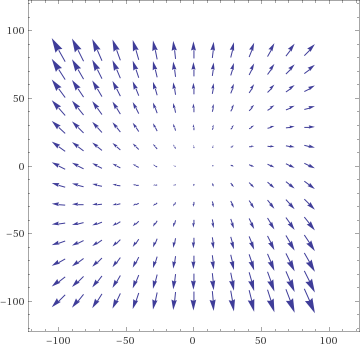
\includegraphics[scale=0.35]{vector_field1}
\end{center}
\end{frame}

%%%%%%%%%%%%%%%%%%%%%%%%%%%%%%%%%%%%%%%%%%%%%%%%%%%%%%%%%%%%%%%%%%%%%%%%%

\begin{frame}{Computer Generated Flow Plot}

Here is a picture of the \emph{flow} of that vector field.

\pause

\begin{center}
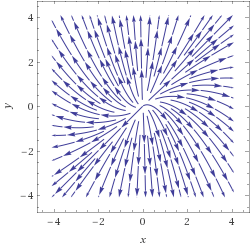
\includegraphics[scale=0.45]{stream1}
\end{center}

\pause

\begin{itemize}
\item The \emph{flow} through a vector field in $\R^2$ is a system of curves
in $\R^2$ such that at each point of the plane, the tangent vector to the
curve at that point is equal to the vector from the vector field at that point.
\item Intuitively, it is the flow that a fluid would take if the fluid were forced
to have a prescribed velocity at each point of the plane.
\end{itemize}
\end{frame}

%%%%%%%%%%%%%%%%%%%%%%%%%%%%%%%%%%%%%%%%%%%%%%%%%%%%%%%%%%%%%%%%%%%%%%%%%

\begin{frame}{Flow of a vector field}


\begin{center}
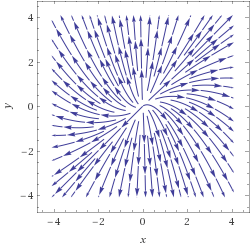
\includegraphics[scale=0.45]{stream1}
\end{center}

\begin{itemize}
\item The flow through a vector field is basically the integral of the vector field.
\item This is something you can learn more about in a class on ordinary differential equations.
\end{itemize}
\end{frame}

%%%%%%%%%%%%%%%%%%%%%%%%%%%%%%%%%%%%%%%%%%%%%%%%%%%%%%%%%%%%%%%%%%%%%%%%%

\begin{frame}{Special directions in the flow of a vector field}


\begin{center}
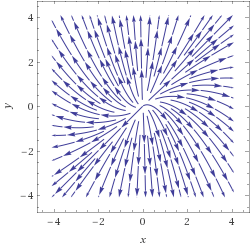
\includegraphics[scale=0.45]{stream1}
\end{center}

\begin{itemize}
\item There are two lines through the origin that are special for this flow. Can you spot them?
\item The line $y=x$ and the $y$-axis. What is special about them?
\item The flow through a point on these lines remains on these lines.
\end{itemize}
\end{frame}

%%%%%%%%%%%%%%%%%%%%%%%%%%%%%%%%%%%%%%%%%%%%%%%%%%%%%%%%%%%%%%%%%%%%%%%%%

\begin{frame}{The special directions are the eigen lines}


\begin{center}
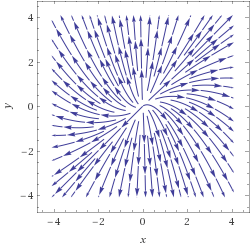
\includegraphics[scale=0.45]{stream1}
\end{center}

\begin{itemize}
\item The special lines in the flow are precisely the eigen lines.
\item $A\bv=\lambda\bv$
\item means that at the point $\bv$ in the plain the velocity of the flow is $\lambda\bv$
\item and so the flow is parallel to the vector $\bv$ itself
\item and so the flow remains on the line through $\bv$.
\end{itemize}
\end{frame}

%%%%%%%%%%%%%%%%%%%%%%%%%%%%%%%%%%%%%%%%%%%%%%%%%%%%%%%%%%%%%%%%%%%%%%%%%

\begin{frame}{Compare with known eigenvector}


\begin{center}
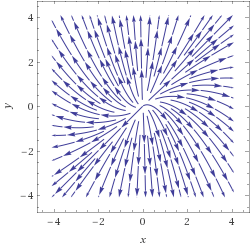
\includegraphics[scale=0.45]{stream1}
\end{center}

\begin{itemize}
\item Earlier we saw that
$
\begin{pmatrix}
1 \\
1
\end{pmatrix}
$
is an eigenvector for our matrix $A$
\item and so is every nonzero vector on the line through
$
\begin{pmatrix}
1 \\
1
\end{pmatrix}
$
\item i.e. the line $y=x$.
\end{itemize}
\end{frame}

%%%%%%%%%%%%%%%%%%%%%%%%%%%%%%%%%%%%%%%%%%%%%%%%%%%%%%%%%%%%%%%%%%%%%%%%%

\begin{frame}{Find a new eigenvector}


\begin{center}
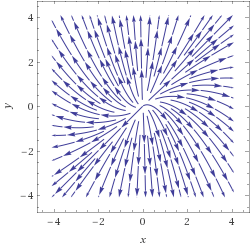
\includegraphics[scale=0.45]{stream1}
\end{center}

\begin{itemize}
\item The flow picture suggests that
$
\begin{pmatrix}
0 \\
1
\end{pmatrix}
$
should also be an eigenvector.
\item
$
\begin{pmatrix}
2 & 0 \\
-1 & 3
\end{pmatrix}
\begin{pmatrix}
0 \\
1
\end{pmatrix}
=
\begin{pmatrix}
0 \\
3
\end{pmatrix}
= 3
\begin{pmatrix}
0 \\
1
\end{pmatrix}
.
$
\item 3 is also an eigenvalue of $A$.
\item
$
\begin{pmatrix}
0 \\
1
\end{pmatrix}
$
is a corresponding eigenvector.
\end{itemize}
\end{frame}

%%%%%%%%%%%%%%%%%%%%%%%%%%%%%%%%%%%%%%%%%%%%%%%%%%%%%%%%%%%%%%%%%%%%%%%%%

\begin{frame}{Computing Eigenvalues and Eigenvectors}


\begin{itemize}
\item How do we find the eigenvalues and eigenvectors of a matrix $A$?
\item We are looking for solutions to the equation $A\bv=\lambda\bv$
where $\bv$ and $\lambda$ are both unknowns.
\item This is not a linear system of equations. So we cannot simply apply Gaussian elimination.
\item The trick is to do the following:
\item Let $I$ be the identity matrix. Then
\item $A\bv=\lambda\bv \SkipImplies A\bv = \lambda I \bv$
\item $\SkipImplies (A-\lambda I) \bv = 0$.
\item We are looking for a nonzero vector $\bv$ and a scalar $\lambda$ such that $(A-\lambda I) \bv = 0$.
\end{itemize}
\end{frame}

%%%%%%%%%%%%%%%%%%%%%%%%%%%%%%%%%%%%%%%%%%%%%%%%%%%%%%%%%%%%%%%%%%%%%%%%%

\begin{frame}{Computing Eigenvalues and Eigenvectors}


\begin{itemize}
\item We are looking for a nonzero vector $\bv$ and a scalar $\lambda$ such that $(A-\lambda I) \bv = 0$.
\item We are looking for a nonzero vector $\bv$ and a scalar $\lambda$ such that $\bv\in\ker(A-\lambda I)$.
\item Notice this implies that $A - \lambda I$ is singular.
\item \textbf{Lemma.} $\lambda$ is an eigenvalue of $A$ iff $(A-\lambda I)$ is singular.
\item $\bv$ is a corresponding eigenvector iff it is in the kernel of $(A-\lambda I)$.
\item This gives us a technique for computing eigenvalues and eigenvectors.
\end{itemize}
\end{frame}

%%%%%%%%%%%%%%%%%%%%%%%%%%%%%%%%%%%%%%%%%%%%%%%%%%%%%%%%%%%%%%%%%%%%%%%%%

\begin{frame}{Computing Eigenvalues}


\begin{itemize}
\item We are looking for a scalar $\lambda$ such that $A-\lambda I$ is singular.
\item We are looking for a scalar $\lambda$ such that $\det(A-\lambda I) = 0$.
\item Notice that if we think of $A$ is a fixed matrix and $\lambda$ as a variable then $\det(A-\lambda I)$ is an
$n$-th degree \emph{polynomial} in $\lambda$.
\end{itemize}
\end{frame}

%%%%%%%%%%%%%%%%%%%%%%%%%%%%%%%%%%%%%%%%%%%%%%%%%%%%%%%%%%%%%%%%%%%%%%%%%

\begin{frame}{Characteristic Polynomial}


\begin{itemize}
\item \textbf{Definition.} Let $A$ be an $n\times n$ matrix. Then
\item $p(\lambda) = \det(A-\lambda I)$
\item is called the \emph{characteristic polynomial} of $A$.
\item It is a polynomial of degree $n$.
\item Example:
\item Let $A=
\begin{pmatrix}
2 & 0 \\
-1 & 3
\end{pmatrix}
$.
\item Compute the characteristic polynomial of $A$.
\item $p(\lambda)=\det(A-\lambda I)$
\item
$
= \det
\begin{pmatrix}
2 - \lambda & 0 \\
-1 & 3 - \lambda
\end{pmatrix}
$
\item
$
= (2-\lambda)(3-\lambda) - 0 = (2-\lambda)(3-\lambda)
$
\item $p(\lambda) = \lambda^2 - 5\lambda + 6$.

\end{itemize}
\end{frame}

%%%%%%%%%%%%%%%%%%%%%%%%%%%%%%%%%%%%%%%%%%%%%%%%%%%%%%%%%%%%%%%%%%%%%%%%%
\begin{frame}{Roots of the characteristic Polynomial}


\begin{itemize}
\item \textbf{Lemma.} Let $A$ be an $n\times n$ matrix. Let
\item $p(\lambda)$ be the characteristic polynomial of $A$.
\item Then $\lambda$ is an eigenvalue of $A$ iff $\lambda$ is a root of $p(\lambda)$.
\item For this reason, another name for eigenvalue is \emph{characteristic root}.
\item Example:
\item Let $A=
\begin{pmatrix}
2 & 0 \\
-1 & 3
\end{pmatrix}
$.
\item $p(\lambda) = \lambda^2 - 5\lambda + 6$
\item
$
= (\lambda-2)(\lambda-3).
$
\item So the characteristic roots of $A$ are 2 and 3.
\item So the eigenvalues of $A$ are 2 and 3.
\end{itemize}
\end{frame}

%%%%%%%%%%%%%%%%%%%%%%%%%%%%%%%%%%%%%%%%%%%%%%%%%%%%%%%%%%%%%%%%%%%%%%%%%
\begin{frame}{Eigenspace}

\begin{itemize}
\item \textbf{Lemma.} Let $T:V\map V$ be a linear transformation and let
$\lambda$ be an eigenvalue for $T$.
\item The set of all eigenvectors corresponding
to $\lambda$ is a nontrivial subspace of $V$ called the \emph{eigenspace} corresponding
to $\lambda$.
\item \textbf{proof.} The eigenspace is just the kernel of $T-\lambda I$ and so
it is a subspace.
\item It is nontrivial because $T - \lambda I$ is singular by definition of eigenvalue. $\qed$
\end{itemize}
\end{frame}

%%%%%%%%%%%%%%%%%%%%%%%%%%%%%%%%%%%%%%%%%%%%%%%%%%%%%%%%%%%%%%%%%%%%%%%%
\begin{frame}{Example of eigenspace}

\begin{itemize}
\item Let $A=
\begin{pmatrix}
2 & 0 \\
-1 & 3
\end{pmatrix}
$.
\item Find the eigenspace corresponding to the eigenvalue $2$.
\item Find the kernel of $A-2I$.
\item Find the kernel of
$
\begin{pmatrix}
0 & 0 \\
-1 & 1
\end{pmatrix}
$
\item To do this we can use Gaussian elimination and back-substitution
\item
$
\begin{pmatrix}
0 & 0 \\
-1 & 1
\end{pmatrix}
\SkipImplies
\begin{pmatrix}
-1 & 1 \\
0 & 0 \\
\end{pmatrix}
$
\item $-x + y = 0 \SkipImplies x = y$.
\item So the eigenspace is is given by
$
\begin{pmatrix}
x \\ y
\end{pmatrix}
=
\begin{pmatrix}
y \\ y
\end{pmatrix}
=
y
\begin{pmatrix}
1 \\ 1
\end{pmatrix}
$
\item In other words, the eigenspace is the 1-dimensional subspace consisting of
all multiples of $\transpose{(1,1)}$.
\item i.e. the line $y=x$.
\end{itemize}
\end{frame}

%%%%%%%%%%%%%%%%%%%%%%%%%%%%%%%%%%%%%%%%%%%%%%%%%%%%%%%%%%%%%%%%%%%%%%%%%
\begin{frame}{Recall the flow plot}


Recall that we can see this 1-dimensional eigenspace on the flow plot.

\pause

\begin{center}
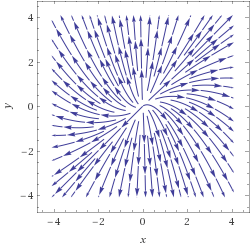
\includegraphics[scale=0.45]{stream1}
\end{center}

\end{frame}

%%%%%%%%%%%%%%%%%%%%%%%%%%%%%%%%%%%%%%%%%%%%%%%%%%%%%%%%%%%%%%%%%%%%%%%%
\begin{frame}{Example of eigenspace}

\begin{itemize}
\item Continuing with $A=
\begin{pmatrix}
2 & 0 \\
-1 & 3
\end{pmatrix}
$.
\item Find the eigenspace corresponding to the eigenvalue $3$.
\item Find the kernel of $A-3I$.
\item Find the kernel of
$
\begin{pmatrix}
-1 & 0 \\
-1 & 0
\end{pmatrix}
$
\item
$
\begin{pmatrix}
-1 & 0 \\
-1 & 0
\end{pmatrix}
\SkipImplies
\begin{pmatrix}
-1 & 0 \\
 0 & 0
\end{pmatrix}
$
\item $-x  = 0 \SkipImplies x = 0$.
\item So the eigenspace is is given by
$
\begin{pmatrix}
x \\ y
\end{pmatrix}
=
\begin{pmatrix}
0 \\ y
\end{pmatrix}
=
y
\begin{pmatrix}
0 \\ 1
\end{pmatrix}
$
\item In other words, the eigenspace is the 1-dimensional subspace consisting of
all multiples of $\transpose{(0,1)}$.
\item i.e. the $y$-axis.
\end{itemize}
\end{frame}

%%%%%%%%%%%%%%%%%%%%%%%%%%%%%%%%%%%%%%%%%%%%%%%%%%%%%%%%%%%%%%%%%%%%%%%%%
\begin{frame}{Recall the flow plot}


Recall that we can see this 1-dimensional eigenspace on the flow plot.

\pause

\begin{center}
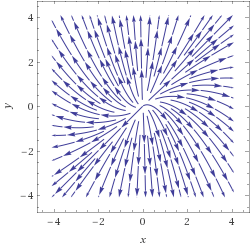
\includegraphics[scale=0.45]{stream1}
\end{center}

\end{frame}

%%%%%%%%%%%%%%%%%%%%%%%%%%%%%%%%%%%%%%%%%%%%%%%%%%%%%%%%%%%%%%%%%%%%%%%%
\begin{frame}{Algebraic and Geometric Multiplicity}

\begin{itemize}
\item \textbf{Definition.} Suppose $A$ is an $n\times n$ matrix and $\lambda$ is an eigenvalue of $A$.
\item The \emph{algebraic multiplicty} of $\lambda$ is the the multiplicty of $\lambda$ as a root
of the characteristic polynomial of $A$.
\item The \emph{geometric multiplicty} of $\lambda$ is the dimension of the eigenspace of $\lambda$.
\item Both values must be between 1 and $n$.
\item Example.  Let
$A=
\begin{pmatrix}
2 & 0 \\
-1 & 3
\end{pmatrix}
$.
\item The eigenvalues of $A$ are 2 and 3.
\item The algebraic multiplicity of both 2 and 3 is one because the characteristic
polynomial of $A$ is $p(\lambda) = (\lambda -2)(\lambda -3)$ and each of 2 and 3
are roots of multiplicty 1 in $p(\lambda)$.
\item The geometric multiplicity of both 2 and 3 is 1 because the eigenspace
both have dimension 1.
\end{itemize}
\end{frame}

%%%%%%%%%%%%%%%%%%%%%%%%%%%%%%%%%%%%%%%%%%%%%%%%%%%%%%%%%%%%%%%%%%%%%%%%
\begin{frame}{Example 2}

\begin{itemize}
\item It's not always the case that the algebraic and geometric multiplicity
of an eigenvalue is the same. Let's look at some other examples.
\item Let
$A=
\begin{pmatrix}
3 & -1 \\
1 & 5
\end{pmatrix}
$.
\item Compute the eigenvalues of $A$ and the corresponding eigenspaces.
\item Compute the algebraic and geometric multiplicity of each eigenvalue.
\item First we compute the characteristic polynomial of $A$.
\item $p(\lambda) = \det(A-\lambda I)$
\item $=\det
\begin{pmatrix}
3 -\lambda & -1 \\
1 & 5 - \lambda
\end{pmatrix}
$
\item $=(3-\lambda)(5-\lambda) + 1$
\item $=\lambda^2 - 8\lambda + 16$
\end{itemize}
\end{frame}

%%%%%%%%%%%%%%%%%%%%%%%%%%%%%%%%%%%%%%%%%%%%%%%%%%%%%%%%%%%%%%%%%%%%%%%%
\begin{frame}{Example 2 continued}

\begin{itemize}
\item $A=
\begin{pmatrix}
3 & -1 \\
1 & 5
\end{pmatrix}
$.
\item The characteristic polynomial is
\item $p(\lambda) =\lambda^2 - 8\lambda + 16$
\item The eigenvalues of $A$ are the roots of $p(\lambda)$.
\item $p(\lambda) = (\lambda - 4)^2$.
\item So $4$ is the only eigenvalue of $A$ and it has algebraic multiplicity 2.
\end{itemize}
\end{frame}

%%%%%%%%%%%%%%%%%%%%%%%%%%%%%%%%%%%%%%%%%%%%%%%%%%%%%%%%%%%%%%%%%%%%%%%%
\begin{frame}{Example 2 continued}

\begin{itemize}
\item $A=
\begin{pmatrix}
3 & -1 \\
1 & 5
\end{pmatrix}
$.
\item There is one eigenvalue, 4, of algebraic multiplicity 2.
\item Now let's find the eigenvectors.
\item Find the null space of $A-4 I=
\begin{pmatrix}
-1 & -1 \\
1 & 1
\end{pmatrix}
$
\item
$
\SkipImplies
\begin{pmatrix}
-1 & -1 \\
0 & 0
\end{pmatrix}
$
\item $-x -y = 0 \SkipImplies x=-y$.
\item $
\begin{pmatrix}
x \\ y
\end{pmatrix}
=
\begin{pmatrix}
-y \\ y
\end{pmatrix}
=
y
\begin{pmatrix}
-1 \\ 1
\end{pmatrix}
$
\item So the eigenspace is 1 dimensional and spanned by $\transpose{(-1, 1)}$.
\item So the geometric multiplicity of $4$ is 1.
\end{itemize}
\end{frame}

%%%%%%%%%%%%%%%%%%%%%%%%%%%%%%%%%%%%%%%%%%%%%%%%%%%%%%%%%%%%%%%%%%%%%%%%%
\begin{frame}{Flow plot 2}


Here is the flow plot for example 2.

\pause

\begin{center}
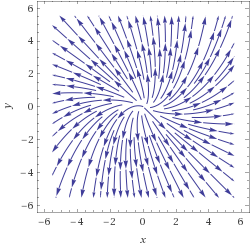
\includegraphics[scale=0.45]{stream2}
\end{center}

\pause

Notice that you can see the 1 dimensional eigenspace: the line $y=-x$.

\end{frame}

%%%%%%%%%%%%%%%%%%%%%%%%%%%%%%%%%%%%%%%%%%%%%%%%%%%%%%%%%%%%%%%%%%%%%%%%
\begin{frame}{Example 3}

\begin{itemize}
\item So far our two examples have been
\item (1) Two eigenvalues of algebraic and geometric multiplicity 1.
\item (2) One eigenvalue of algebraic multiplicity 2 but geometric multiplicity 1
\item Let's look at a different example
$I=
\begin{pmatrix}
1 & 0 \\
0 & 1
\end{pmatrix}
$.
\item Compute the eigenvalues of $I$ and the corresponding eigenspaces.
\item Compute the algebraic and geometric multiplicity of each eigenvalue.
\item First we compute the characteristic polynomial of $I$.
\item $p(\lambda) = \det(I-\lambda I)$
\item $=\det
\begin{pmatrix}
1 -\lambda & 0 \\
0 & 1 - \lambda
\end{pmatrix}
$
\item $=(1-\lambda)^2$
\end{itemize}
\end{frame}

%%%%%%%%%%%%%%%%%%%%%%%%%%%%%%%%%%%%%%%%%%%%%%%%%%%%%%%%%%%%%%%%%%%%%%%%
\begin{frame}{Example 3 continued}

\begin{itemize}
\item The characteristic polynomial of the identity matrix $I$ is
$p(\lambda) = (1-\lambda)^2$
\item So there is only one eigenvalue, 1, and it has algebraic multiplicity 2.
\item To find the eigenspace, we need to find the kernel of $I - 1 I$.
\item This is the kernel of the zero matrix.
\item So the eigenspace is all of $\R^2$.
\item So the identity matrix has one eigenvalue, 1, of algebraic and
geometric multiplicity 2.
\end{itemize}
\end{frame}

%%%%%%%%%%%%%%%%%%%%%%%%%%%%%%%%%%%%%%%%%%%%%%%%%%%%%%%%%%%%%%%%%%%%%%%%%
\begin{frame}{Flow plot 3}


Here is the flow plot for example 3.

\pause

\begin{center}
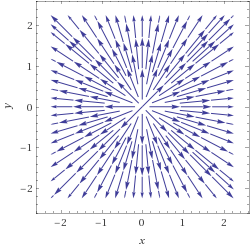
\includegraphics[scale=0.45]{stream3}
\end{center}

\pause

Notice that you can see the 2 dimensional eigenspace: Every vector in $\R^2$ is an eigenvector.

\end{frame}

%%%%%%%%%%%%%%%%%%%%%%%%%%%%%%%%%%%%%%%%%%%%%%%%%%%%%%%%%%%%%%%%%%%%%%%%
\begin{frame}{Example 4}

\begin{itemize}
\item So far our three examples have been
\item (1) Two eigenvalues of algebraic and geometric multiplicity 1.
\item (2) One eigenvalue of algebraic multiplicity 2 but geometric multiplicity 1
\item (3) One eigenvalue of algebraic and geometric multiplicity 2.
\item Let's look at a different example.
\item
$A=
\begin{pmatrix}
1 & -1 \\
1 & 1
\end{pmatrix}
$.
\item First we compute the characteristic polynomial of $A$.
\item $p(\lambda) = \det(A-\lambda I)$
\item $=\det
\begin{pmatrix}
1 -\lambda & -1 \\
1 & 1 - \lambda
\end{pmatrix}
$
\item $=(1-\lambda)^2 + 1$
\item $=\lambda^2-2\lambda + 2$
\end{itemize}
\end{frame}

%%%%%%%%%%%%%%%%%%%%%%%%%%%%%%%%%%%%%%%%%%%%%%%%%%%%%%%%%%%%%%%%%%%%%%%%
\begin{frame}{Example 4, Continued}

\begin{itemize}
\item $A=
\begin{pmatrix}
1 & -1 \\
1 & 1
\end{pmatrix}
$.
\item The characteristic polynomial of $A$ is
$p(\lambda) = \lambda^2-2\lambda + 2$
\item Find the roots of $p(\lambda)$
\item
$$
\lambda = \frac{2 \pm \sqrt{4 - 8}}{2}
$$
\item
$$
 = \frac{2 \pm 2\sqrt{-1}}{2} = 1 \pm i.
$$
\item So $A$ has two eigenvalues but they are \emph{not real}!
\item Notice that they are complex conjugates.
\item \textbf{Lemma} Let $A$ be a real $n\times n$ matrix. Then some of the
eigenvalues of $A$ may be non-real complex numbers.
\item But the non-real eigenvalues must occur in complex conjugate pairs.
\item That is, if $z$ is an eigenvalue then $\zbar$ is also an eigenvalue.
\end{itemize}
\end{frame}

%%%%%%%%%%%%%%%%%%%%%%%%%%%%%%%%%%%%%%%%%%%%%%%%%%%%%%%%%%%%%%%%%%%%%%%%
\begin{frame}{Non-real eigen pairs}

\begin{itemize}
\item What could it mean for $A$ to have a non-real eigenvalue $\lambda$?
\item An eigenvalue is supposed to satisfy $A\bv=\lambda v$ for some eigenvector $\bv$.
\item But if $\bv\in\R^n$ then $A\bv\in\R^n$,
\item whereas if $\lambda\notin\R$ then $\lambda\bv\notin\R^n$.
\item \textbf{Lemma} Let $A$ be a real $n\times n$ matrix.
\item Suppose that $A$ doesn't have any real eigenvalues.
\item Then $A$ doesn't have any real eigenvectors.
\end{itemize}
\end{frame}


%%%%%%%%%%%%%%%%%%%%%%%%%%%%%%%%%%%%%%%%%%%%%%%%%%%%%%%%%%%%%%%%%%%%%%%%%
\begin{frame}{Flow plot 4}


Here is the flow plot for example 4.

\pause

\begin{center}
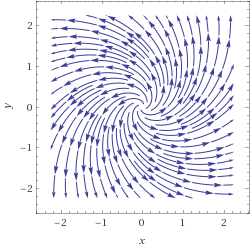
\includegraphics[scale=0.45]{stream4}
\end{center}

\pause

Notice that you can see that there are no eigenvectors in $\R^2$.
\pause

But this only means there are no \emph{real} eigenvectors. In complex space
we do have eigenvectors.
\end{frame}

%%%%%%%%%%%%%%%%%%%%%%%%%%%%%%%%%%%%%%%%%%%%%%%%%%%%%%%%%%%%%%%%%%%%%%%%%
\begin{frame}{Complex matrices}

\begin{itemize}
\item Because we must confront the fact that a real matrix may have complex eigenvalues,
\item even if we only care about $\R^n$, we are forced to consider vectors and matrices over $\C$.
\item Everything that we have learned in the class so far about vectors and matrices and vector spaces and linear transformations over $\R$
\item applies equally well to vectors and matrices and vector spaces and linear transformations over $\C$.
\item When working over $\C$ you allow your scalars to be complex numbers.
\item You allow the entries in your matrices and vectors to be complex numbers.
\item But everything else (for example how you multiply two matrices together) works the same way.
\item With one exception: Inner-products must be dealt with differently over
complex vectors spaces.
\end{itemize}
\end{frame}


\end{document}


